\documentclass[professionalfont]{beamer}

\usepackage{graphicx}
\usepackage{newtxtext,newtxmath}
\usetheme{default}
\usecolortheme{seagull}

\setbeamertemplate{navigation symbols}{}
\setbeamertemplate{itemize item}{\textbullet} 
\setbeamertemplate{title page}{
    \begin{center}
        {\textcolor{blue}{\textbf{\fontsize{12}{14}\selectfont MapCoder: Multi-Agent Code Generation\\for Competitive Problem Solving}}} \\[1.5cm]
        
        {\fontsize{9}{14}\selectfont Md. Ashraful Islam, et al \\[0.3cm]
        Bangladesh University of Engineering and Technology \\[0.3cm]
        May 18, 2024}
    \end{center}
}
% ------------------ Title ------------------

\begin{document}
\frame{\titlepage}


\begin{frame}
\begin{center}
    { \textbf{\textcolor{blue}{ {\fontsize{12}{14}\selectfont Abstract} }} }
\end{center}
\\[0.5cm]

{\fontsize{10}{14}\selectfont 
\begin{itemize}
    \item LLMs have limited ability for coding
    
    - Code generation is harder than just NLP
\end{itemize}
\\[0.5cm]

\begin{itemize}
    \item New framework MapCoder, which has 4 stages
    
    - Retrieval, Planning, Coding, Debugging
    
    - It is open source
\end{itemize}
}

\end{frame}
% ------------------ Slide 1 ------------------

\begin{frame}
\begin{center}
    { \textbf{\textcolor{blue}{ {\fontsize{12}{14}\selectfont Previous works} }} }
\end{center}

{\fontsize{10}{14}\selectfont 
\begin{itemize}
    \item Chain-of-Thought
    
    - Pseudo code-based generation
    
    - Fail to pass test cases, No bug fixing
\end{itemize}

\begin{itemize}
    \item Retrieval-based approach
    
    - Leverage relevant problems and solutions
    
    - Fail to pass test cases, No bug fixing
\end{itemize}

\begin{itemize}
    \item Self-reflection
    
    - Iteratively evaluates generated code against test case
    
    - Only leverage the problem description itself in a zero-shot manner
\end{itemize}
}

\end{frame}
% ------------------ Slide 2 ------------------

\begin{frame}
\begin{center}
    { \textbf{\textcolor{blue}{ {\fontsize{12}{14}\selectfont Multi Agent Prompting Coder} }} }
\end{center}

{\fontsize{10}{14}\selectfont 
\begin{itemize}
    \item Retrieval agent
    
    - Generates relevant examples itself
\end{itemize}

\begin{itemize}
    \item Dynamic Traversal Block
    
    - Plans and considers the confidence of the generated plans
    
    - Code generation and debugging
\end{itemize}
}

\begin{center}
    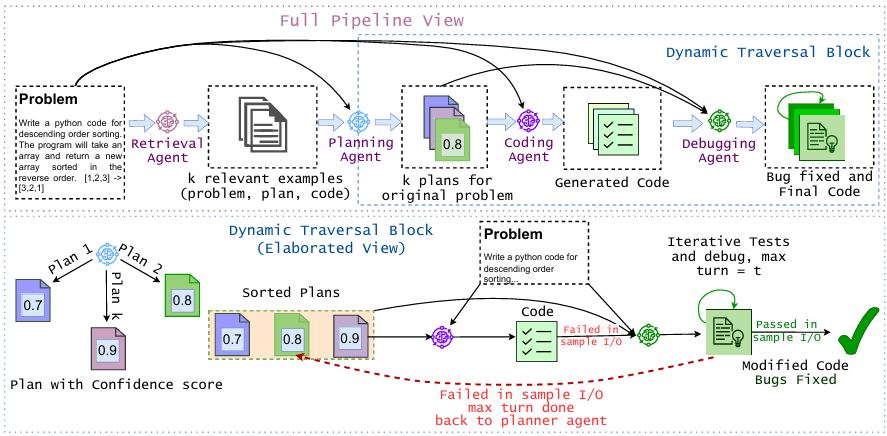
\includegraphics[width=1.0\textwidth]{figure1.png}
\end{center}

\end{frame}
% ------------------ Slide 3 ------------------

\begin{frame}
\begin{center}
    { \textbf{\textcolor{blue}{ {\fontsize{12}{14}\selectfont Experiment} }} }
\end{center}

{\fontsize{10}{14}\selectfont 
\begin{itemize}
    \item 5 basic-level benchmark + 3 contest-level benchmark
    \item GPT-3.5-Turbo and GPT-4 as foundation models
    \item Various prompting baselines including MapCoder
\end{itemize}
}

\begin{center}
    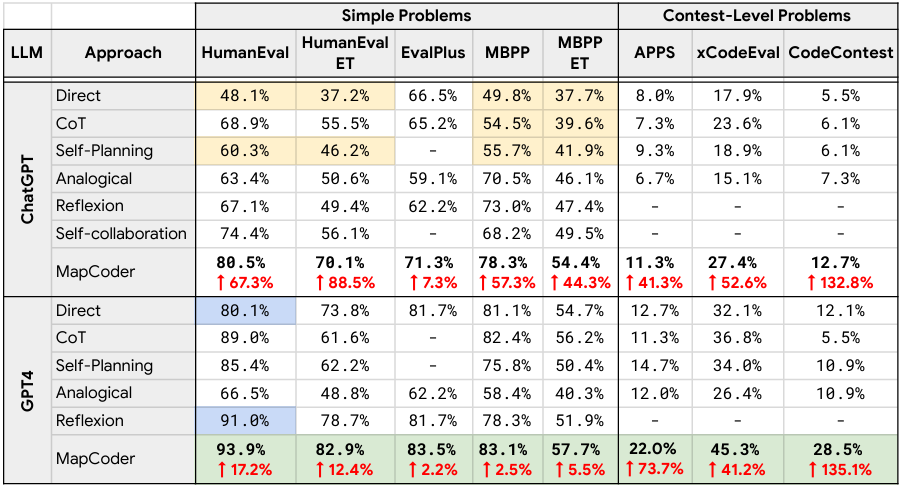
\includegraphics[width=1.0\textwidth]{table2.png}
\end{center}

\end{frame}
% ------------------ Slide 4 ------------------

\begin{frame}
\begin{center}
    { \textbf{\textcolor{blue}{ {\fontsize{12}{14}\selectfont Experiment Results} }} }
\end{center}

{\fontsize{10}{14}\selectfont 
\begin{itemize}
    \item Performance gain on varying difficulty levels
    \item Performance gain on different programming languages
\end{itemize}
}

\begin{center}
    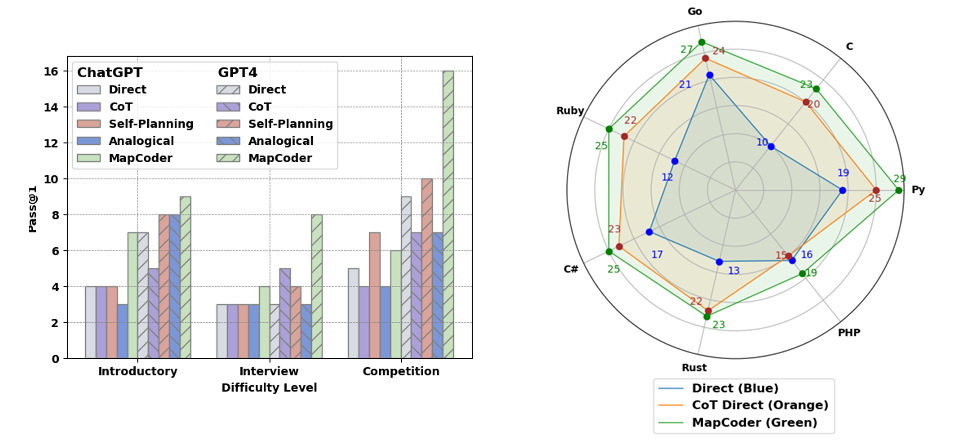
\includegraphics[width=1.0\textwidth]{figure6.png}
\end{center}

\end{frame}
% ------------------ Slide 5 ------------------

\begin{frame}
\begin{center}
    { \textbf{\textcolor{blue}{ {\fontsize{12}{14}\selectfont Ablation study} }} }
\end{center}
\\[0.5cm]

{\fontsize{10}{14}\selectfont 
\begin{itemize}
    \item Removed each agent
    
    - Showed that every agent has its role in the pipeline

    - Debugging Agent has the most significant impact
\end{itemize}
}
\\[0.5cm]

\begin{center}
    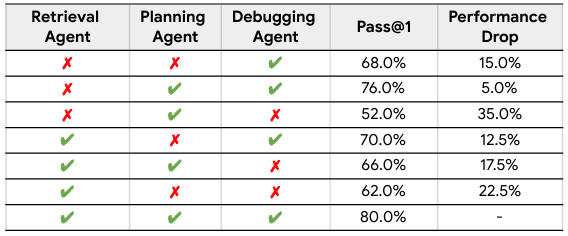
\includegraphics[width=0.8\textwidth]{table6.png}
\end{center}

\end{frame}
% ------------------ Slide 6 ------------------

\begin{frame}
\begin{center}
    { \textbf{\textcolor{blue}{ {\fontsize{12}{14}\selectfont Conclusion} }} }
\end{center}
\\[0.5cm]

{\fontsize{10}{14}\selectfont 
\begin{itemize}
    \item MapCoder outperformed many SOTA approaches
    
    - Performance gain on varying difficulty levels

    - Performance gain on different programming languages
\end{itemize}
\\[0.5cm]

\begin{itemize}
    \item Limitation
    
    - It generates a large number of tokens
    
    - Challenging in resource-constrained environment
\end{itemize}
}
\end{frame}
% ------------------ Slide 7 ------------------

\end{document}
